\subsection{Region Transition Probability}

A travel path of a taxi can be simplified as a multi-hop process, in which a hop indicates an load/drop event happened. Seeing that, we define a \emph{ region transition probability} to figure out the probability of the next hop falling in a certain region $R_j$ from the current region $R_i$. Particularly, when two successive events are different: one load and one drop. Therefore, the region $R_i$ and $R_j$ are recognized by different metrics, that is, drop or load event distribution. For an instance, if the taxi is currently occupied, then the next hop event is the drop one. Hence, choosing a target region from a region set obtained based on drop event distribution is more logical.
%%ÿ���ֲ���ͷһ��Ҫ��&���ţ�����\qquad Ϊ��ո�����

Before defining the region transition probability, we first describe our \textbf{region recognition process}.
Firstly, we divide the area into $100\times 100$ small grids, and define them as cells (as shown in the following equation) where $lon$ and $lat$ are relevant longitude and latitude, $len_x$ and $len_y$ are side length of the grid/cell). 
\[C_{x,y}::=\{(lon,lat)|x \le \frac{{lon}}{{len_x}} < x + 1,
y \le \frac{{lat}}{{len_y}} < y + 1\}.\]
Then, we consider a region as a union of adjacent cells, as following.
\[R_m:: = \{ C_{x,y}|\exists C_{i,j} \in R_m
\Rightarrow \|x - i\| \le 1,\|y - j\| \le 1\}.\]
The main idea of clustering cells to regions is to put adjacent cells with event density larger than an event threshold $\eta$ into a same region. To avoid the size of a region become too large or too small, we set a limitation on the size of a region, say $\|R_i\|\leq ClusterSize$, and also limit the number of final region is less than or equal to $200$. Thus, we only consider the top $200$ regions, in which $C_{x,y}.events\geq \eta$. After that, the other cells, who do not belong to the top 200 regions, will also be clustered into the $200$ regions, while $\|R_j\|\leq ClusterSize$. The overall clustering algorithm is simple. We sort the $100\times 100$ cells by event density in descending order, and begin with the first cell to search its neighbors whether to join the same region using breadth traversal. Consequently, every cells will be clustered into regions and the size of every region is not larger than $ClusterSize$. 
By clustering cells into regions, two region sets, $\textbf{R}^{load}$ and $\textbf{R}^{drop}$, can be recognized from the data set. The region recognition results for load/drop events are shown in Fig.~\ref{figure_region_recognizition} for the Beijing taxi data set.
In this figure, every colored block presents a region. In addition, $ClusterSize=200$, and $\eta=121$ for load event and $\eta=141$ for drop event ( these are set by the average event density of the top $5000$ cells order by its event density). You can see clearly differences among load region and drop-off regions.

\begin{figure}[!t]
\centering
\subfigure[drop event regions]{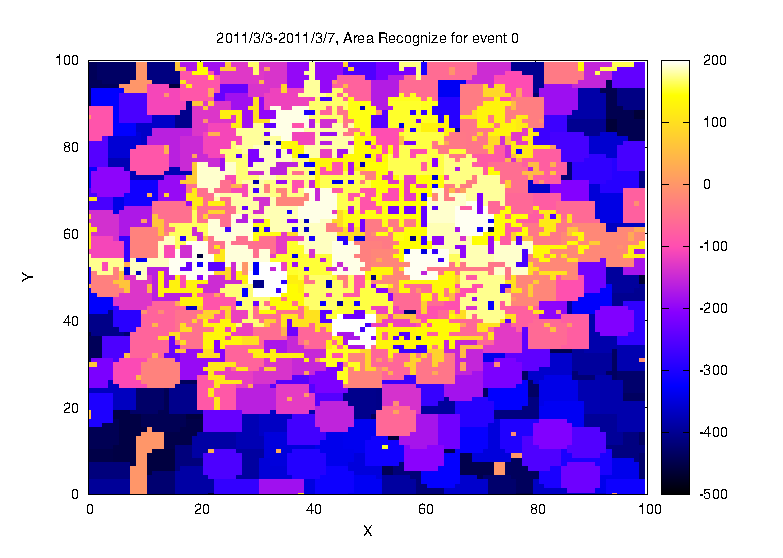
\includegraphics[width=0.23\textwidth]{figures_201103/region/Areas-2011_event0.eps}}
\subfigure[load event regions]{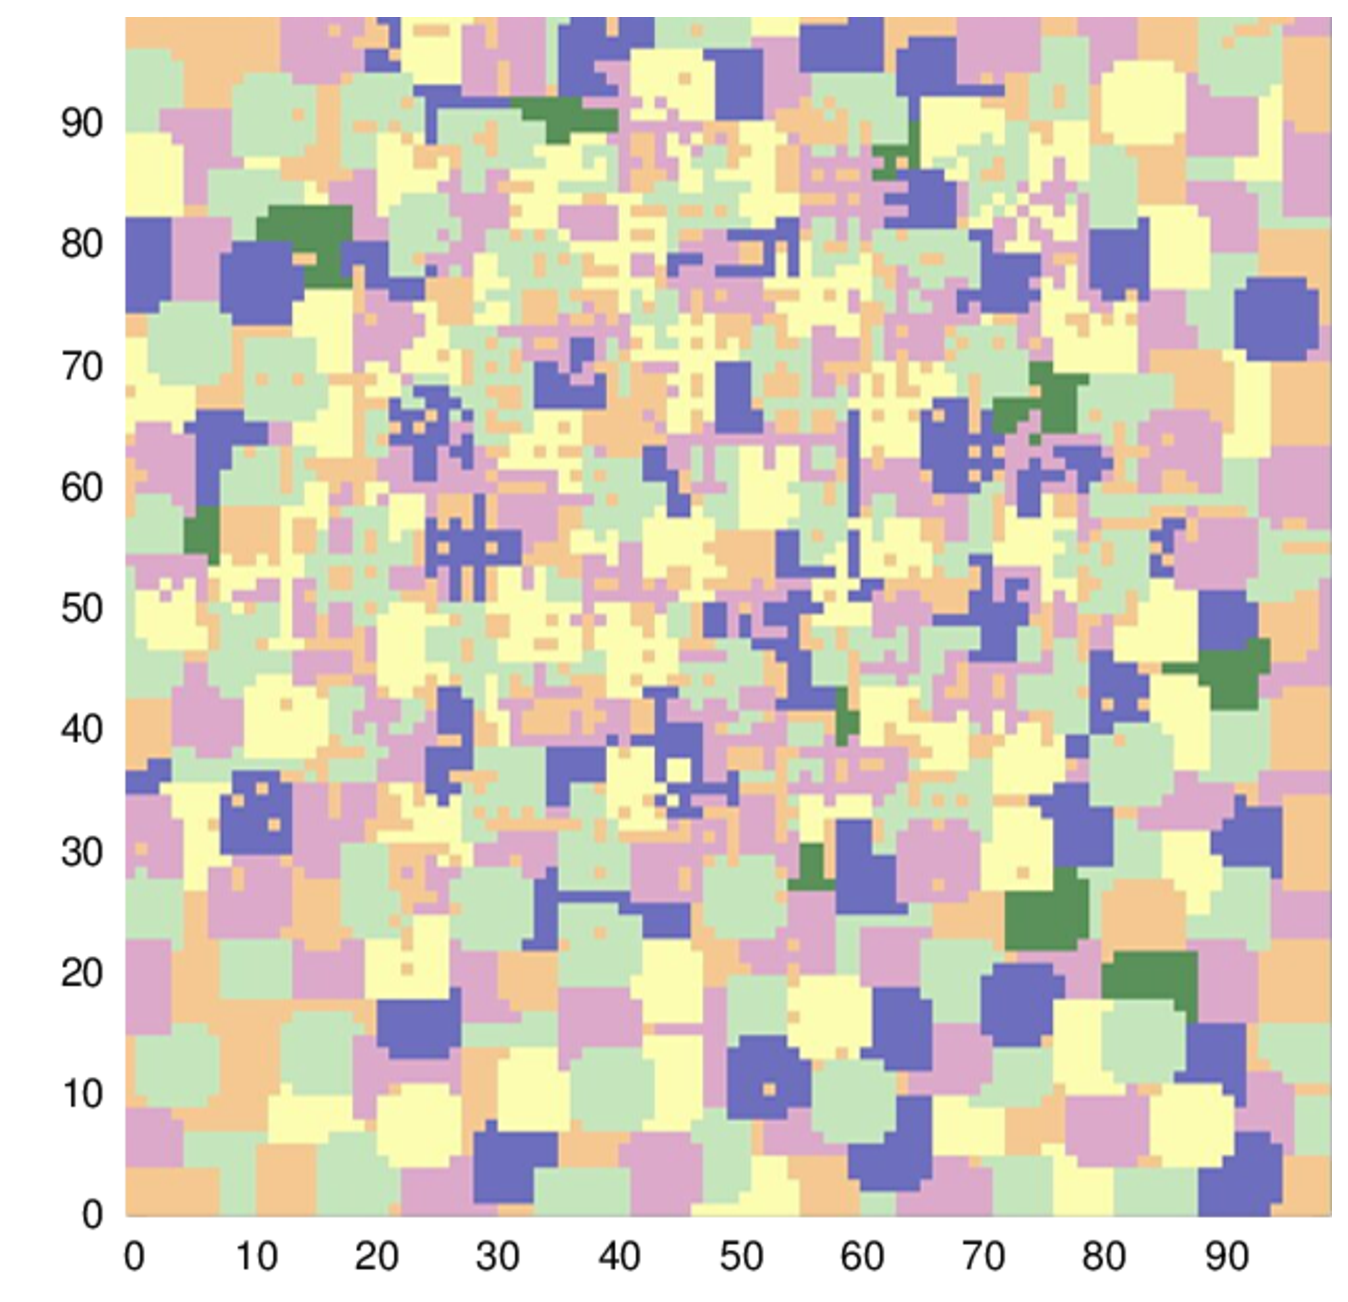
\includegraphics[width=0.23\textwidth]{figures_201103/region/Areas-2011_event1.eps}}
\centering
\caption{Region recognition}\label{figure_region_recognizition}
\end{figure}

\textbf{Calculation of region transition probability}: After clustering cells into regions, the transition probability from $R_i^{load}$ to $R_j^{drop}$ and the one from $R_i^{drop}$ to $R_j^{load}$, donated as $p_{i\rightarrow j}^{load\rightarrow drop}$ and $p_{i\rightarrow j}^{drop\rightarrow load}$, can be caculated. Since both transition probability can be calculated similarly, we only introduce the detailed one of $p_{i\rightarrow j}^{load\rightarrow drop}$. 

First, we count all records in $R_i^{load}$ from the data set,  i.e. $REC_i^{load}=\{r~|~r.location\in{R_i^{load} \textit{ and }  r.event=load}\}$. Let $\|REC_i^{load}\|$ be the amount of such records. For record $r \in REC_i^{load}$, the next event and location can be easily obtained from the data set. Thus, we can get the set of such records whose next event is drop and next location is $R_j^{drop}$, i.e., $REC_{i\to j}^{load\to drop}=\{r~|~r.event=load,~r.event_{next}=drop,~r.location_{current}\in R_i^{load}, \textit{ and }  r.location_{next}\in R_j^{drop}\}$. Let $\|REC_{i\to j}^{load\to drop}\|$ be the amount of such records. We can then easily obtain the transition probability from $R_i^{load}$ to $R_j^{drop}$, as follows,
\[p_{i \to j}^{load \to drop} = \frac{\|REC_{i\to j}^{load\to drop}\|}{\|REC_i^{load}\|.}\]


%\begin{equation}\label{transition_matrix}
%  P^{load\to drop} = (p_{i\to j}^{load\to drop})_{m\times n}
%\end{equation}

%\begin{equation}\label{transition_matrix}
%  P^{drop\to load} = (p_{i\to j}^{drop\to load})_{n\times m}
%\end{equation}

%%\begin{equation}\label{equation_taxiset_matrix}
%\textbf{\emph{P^{on\to drop}}}=(p_{i\to j}^{load\to drop})_{m*n}\\
%\textbf{\emph{P^{drop\to load}}}=(p_{i\to j}^{drop\to load})_{n*m}\\
%\end{equatiload}

